\chapter{电磁感应}
\minitoc[n]
\section{教学要求}
这一章教材是以初中学过的电磁现象以及高中学过的电
场、磁场等知识为基础,阐述电磁感应现象和电磁感应的基本
规律。这些内容是电磁学的基础知识,也是学习交流电、电磁
振荡和电磁波的基础。

本章教材可分为四个单元。课文的第一节为第一单元,
讲述电磁感应现象。第二、三节为第二单元,讲述楞次定律。第
四、五节为第三单元,讲述法拉第电磁感应定律和电磁感应现
象中的能量转化问题。第六节至第九节为第四单元,讲述电磁
感应现象中的几种特殊情况。

本章教材以法拉第电磁感应定律为中心,进一步揭示了
电与磁的内在联系,因而法拉第电磁感应定律是这一章的重
点。楞次定律及其应用,法拉第电磁感应定律的应用,是教
学上的难点。

用磁通量的概念来概括和表达电磁感应现象的规律,是
这一章的特点。教材是用磁通量的变化来叙述感生电流的产
生条件和楞次定律,用磁通量的变化率来叙述法拉第电磁感
应定律的。因此,理解磁通量的变化和磁通量的变化率的意
义,了解它们之间的区别与联系,对于学好全章具有重要的
意义。

研究感生电流产生的条件、判定感生电流的方向、确定感
生电动势的大小,都是通过实验分析得出规律的。因此在教
学中,做好实验是非常重要的。

用磁通量的变化来表述楞次定律,可适用于电磁感应现
象的各种情况,因而具有普遍性。在教学中,要注意强调这一
点。但是,对于由相对运动而产生感生电流的情形,用阻碍相
对运动来表述楞次定律,用起来比较方便,特别是在分析电磁
感应现象中的能量转化时要用到。因此,在教材中也注意了这
种情况下楞次定律的表述。学习楞次定律要着重使学生学会
运用这个定律来判断感生电流及其磁场的方向。学生已经学
过用右手定则判断感生电流的方向,教学中应该使学生理解
在由相对运动(导体切割磁力线)而引起的电磁感应现象中,
用右手定则和用楞次定律来判断感生电流的方向,结果是一
致的。

感生电动势是表示电磁感应现象的重要物理量,是电磁
学的基本概念,应使学生掌握。教材不要求区别感生电动势
和动生电动势,不要求学生掌握内电路中各点电势的高低。感
生电动势的大小,教材表述为$\mathcal{E}=k\dfrac{\Delta\phi}{\Delta t}$,
,而没有在等式的右边
加上“$-$”号,这是因为,对一般学生,理解负号的意义比较
困难。

能的转化和守恒定律,是普遍适用的客观规律。楞次定
律和法拉第电磁感应定律也符合这一规律。教材只就由相对
运动产生的电磁感应现象来分析能的转化和守恒问题,对于
没有相对运动而磁场变化的情形,由于能的转化涉及场能,而
没有加以分析。

直流电动机的反电动势是选讲教材,反电动势的概念在
讲变压器时要用到。这节内容,可以使学生知道电磁感应现
象不是孤立发生的,通电线圈在磁场中受力而运动,同时就切
割磁力线,产生电磁感应现象,出现反电动势。这个反电动势
又反过来影响线圈中的电流和线圈受力情况、运动情况。这
节内容对培养学生综合分析问题的能力是有好处的。如果课
时允许,希望讲一下这节教材。

自感现象是电磁感应现象的特殊情况,这个内容是学习
交流电、电磁振荡等内容的基础。教学中,要注意讲清自感系
数的物理意义。在自感现象的应用中,要讲清日光灯的两个
主要元件-起动器和镇流器的工作原理和作用。还可结合
实际情况,补充讲解一些日光灯的使用维修知识。

涡流一节是选讲教材,使学生知道产生涡流的条件,对
涡流的有利、有害两方面有所了解就可以了,不要求作进一步
的讨论。

本章的教学要求是:
\begin{enumerate}
\item 理解电磁感应现象,掌握产生感生电流的条件.
\item 掌握楞次定律和右手定则,并会应用它们判断感生电
流的方向。
\item 掌握法拉第电磁感应定律,并能用来计算有关感生电
动势的问题。
\item 理解自感现象及其在实际中的应用,理解自感电动势
的概念和自感系数的物理意义。
\end{enumerate}

\section{教学建议}
\subsection{电磁感应现象}
这一单元研究感生电流产生的条件,是本章教材的起始
课。教学时要注意从复习电生磁以及磁场对电流的作用这样
一些电与磁相互联系的已有知识中提出问题,即引导学生研
究如何利用磁场来获得电流的问题。同时可以简要介绍法拉
第其人及其在物理学上的贡献,以激发学生的学习积极性。

\subsubsection{感生电流产生的条件}
课本中安排了三个演示实验,它是本单元中研究感
生电流产生条件的依据,也是后面研究楞次定律、法拉第电磁
感应定律的基础。因此,认真做好三个演示实验,力争有较好
的观察效果,是教学的关键。同时,要引导学生逐步从实验
现象中总结出正确的结论,这不但是学生掌握概念和规律的
需要,而且也有利于培养学生的抽象概括能力。

三个实验的观察重点不同.实验一是观察闭合电路
的一部分导体在磁场中运动时产生感生电流的条件。这里要
引导学生注意观察导体向上或向下运动和向左或向右运动的
不同结果,从而了解“导体做切割磁力线运动”的含义。可以
明确告诉学生,所谓切割磁力线的运动,就是导体运动速度的
方向和磁感应强度的方向不平行,这也为推导$\mathcal{E}=B\ell v\sin\theta$
这一公式打下基础。实验二是进一步观察导体不动而磁铁运
动时是否产生感生电流。从而使学生了解,只要导体和磁场
之间发生切割磁力线的相对运动,闭合电路中就会产生感生
电流,这里要强调相对运动必须是导体切割磁力线的,否则
闭合电路中是没有感生电流的。实验三是研究导体静止在
磁场中时能否获得感生电流的问题。在这个实验里,学生能
观察到不论是线圈$A$电路的接通或断开还是变阻器滑动片的
移动,线圈$B$电路中都出现感生电流。在观察实验现象的基
础上,要引导学生分析上述现象的物理过程,在上一章的学习
中,学生已经知道由电流所激发的磁场的磁感应强度$B$总是
正比于电流强度$I$的,即$B\propto I$是一个有普遍意义的关系。
电路的闭合或断开控制了电流从无到有的变化,变阻器则是
通过改变电阻来改变电流。而电流的变化必将引起磁场的
变化,线圈$B$中出现感生电流就是由穿过它所围面积的磁场
变化所引起的。

\subsubsection{结论}

教材是在每个演示实验的后面,对实验现象加
以分析,通过对三个实验的分析,逐步得出产生感生电流的
条件,这就是:“不管是闭合电路的一部分导体做切割磁力线
的运动,还是闭合电路中的磁场发生变化,穿过闭合电路的
磁力线条数都发生变化,这时闭合电路中就有感生电流
产生。”然后,再用磁通量的概念总结出只要穿过闭合电路的
磁通量发生变化,闭合电路中就会产生感生电流这个 一般
条件。

处理这段教材时应注意以下几点:

通过提问学生来复习磁通量的概念,明确磁通量的
定义式为$\phi=BS\cos\theta$, $\theta$为面积$S$与垂直于磁感应强度方向
平面的夹角。当$S$与$B$垂直时,$\phi=BS$. 复习磁通量的概念之
后,可向学生提出“根据磁通量的定义式来分析,使一个面积
为$S$的闭合线圈中的磁通量发生变化,有哪几种方法”的问题,
以使学生进一步明确通过一闭合面积的磁通量是由哪些因
素决定的,同时为总结概括产生感生电流的条件打下基础。

利用磁通量概念概括产生感生电流的条件时,要注
意强调磁通量的变化。教学时,可画出上述三个实验的示意
图,并将它们的磁力线的分布在图上表示出来,如图2.1中
甲、乙、丙所示。
\begin{figure}[htp]
    \centering
\includegraphics[scale=.6]{fig/2-1.png}    
    \caption{}
\end{figure}

在图2.1甲中,闭合电路的一部分导体$AB$向右或向左
运动时都作切割磁力线运动,通过闭合电路的磁力线条数发
生了或增或减的变化.磁通量的变化量$\Delta\phi=B\Delta S$. 在图2.1
乙中,当$N$极向下插入线圈时,由于离$N$极近处磁感应强度较
大,使得线圈内部空间的磁感应强度变大。而线圈的面积不
变,故通过线圈的磁通量增加,图2.1丙中,接通开关$K$的瞬
间,线圈$A$中的电流由无到有,故磁感应强度由零开始增大,
而线圈$A$的面积$S$不变,所以磁通量也由零开始增大。上面
两个实验中,磁通量的变化$\Delta\phi=\Delta B\cdot S$. 通过上述分析,应使学生认识到:不论是导体作切割磁力线运动,还是磁场发生
变化,实质上都是引起穿过闭合电路的磁通量发生变化。在
此基础上给学生明确指出,产生感生电流的条件可以归结为
“穿过闭合电路的磁通量发生变化”。

因为初中教材中只讲了切割磁力线的情况,给学生
留下了一个先人为主的印象。又由于在某些情况下利用切割
磁力线来分析感生电流比较方便,因此,学生习惯于利用切割
磁力线来判断电磁感应现象,为了使学生对于用磁通量观点
来判断电磁感应现象加深认识,可通过一些典型例题让学
生进行讨论.例如课本中练习一4就可以放在课堂上处理。
通过例题分析还应使学生认识到,掌握磁体和通电导体所产
生的磁场的特点及磁力线在空间的分布情况,在判断感生电
流时也是十分重要的。


\subsubsection{培养学生用实验研究问题的能力}

在学校实验器
材较全且学生水平比较整齐的情况下,可采取在课堂上学生
随老师一起做实验的办法来组织这一节的教学,这样可对感
生电流产生的条件获得深刻的印象。

\subsection{楞次定律}
楞次定律是确定感生电流方向的一般规律。由于它的内
容抽象,涉及到电与磁间复杂的相互关系,因此它是本章教材
的一个难点。

试用本是从能量守恒定律出发,通过推理得出楞次定律
的。但是从能量守恒定律得出的是阻碍相对运动,要得出阻
碍磁通量变化的表达,还需要进一步的讲解。这就使楞次
定律的得出显得不够轻快。为了解决这个问题,本单元教材
抓住了磁通量变化这个线索,尽可能简捷地引出楞次定律。至
于电磁感应现象中的能量守恒问题,放在第三单元中去讨论。

本单元的重点是使学生明确引起感生电流的磁通量
的变化和感生电流所激发的磁场之间的关系。为了解决这个
问题,可先复习学生所学过的知识:
\begin{enumerate}
\item 磁通量的变化是产生感
生电流的条件。  
  \item 根据电流的磁效应,感生电流一定会激发
磁场,感生电流的方向与它所激发的磁场的方向间的关系可
由右手定则来判定.
\end{enumerate}
在上述知识基础上,再向学生提出“磁通
量的变化与感生电流的磁场之间有什么关系”的问题,并通过
实验引导学生来研究。

在利用课本图2.2所示的装置做实验时,要注意:
\begin{enumerate}
\item 
明确线圈导线的绕向(实验用的线圈最好是实验者自己绕制
的).   
 \item 实验前,要用旧干电池来确定电流的方向与电流表
指针偏转方向的关系。
\end{enumerate}

实验时,最好能将磁铁磁场的磁通量的变化以及感生电
流所激发的磁场的磁力线方向简明示出,使学生能顺利地找
出二者之间的关系。可将实验中观察到的现象填入下表。
\begin{center}
\begin{tabular}{c|p{.08\textwidth}p{.08\textwidth}p{.08\textwidth}p{.13\textwidth}p{.08\textwidth}c}
    \hline
   & 原磁场方向  & 原$\phi$变化情况& 感生电流方向& 感生电流磁场$B$方向& $B$与$\phi$的关系& 结论\\
   \hline
   $N$极向上\\
   $N$极向下\\
   $S$极向上\\
   $S$极向下\\
   \hline
\end{tabular}
\end{center}

为使学生更加形象地了解感生电流的磁场B和原磁场磁
通中的关系,分析实验结果时要注意强调:原磁场的磁通量
减少时,感生电流磁场与原磁场方向相同;原磁场的磁通量
增加时,感生电流磁场与原磁场方向相反,然后使学生进一
步认识,感生电流是通过其磁场与原磁场同方向或反方向来
起到阻碍磁通量变化的作用的。

\subsubsection{楞次定律的表述}

楞次定律表述为:“感生电流具有这样的方向,就是
感生电流的磁场总要阻碍引起感生电流的磁通量的变化。”虽
然这一表述是建立在实验的基础上,但为避免学生产生误解,
要针对学生容易产生的误解作一些讲解。①学生往往把“阻碍
原磁场的变化”理解为“阻碍原磁场”,从而得出“感生电流的
磁场必与原磁场的方向相反”,或者“感生电流的流向必与原
来电流的流向相反”等错误结论。②学生往往把“阻碍原磁场
的变化”理解为“阻止原磁场的变化”,从而得出“有了感生电
流,原磁场就不会变化了”或“感生磁场加原磁场等于稳恒磁
场”等错误结论。在实际教学时,应根据学生的实际问题,有
针对性的讲解,使学生真正理解楞次定律上述表述的意义。

教材通过分析磁铁和通电螺线管之间的磁极相互作
用,提出了楞次定律的另一种表述,即导体和磁体发生相对运
动时,感生电流总要阻碍相对运动。应该告诉学生,这是从不
同角度表述同一个定律,而不是两个定律。

\subsubsection{楞次定律的应用}
这一节的教学,要使学生通过实例的分析,加深对楞
次定律的理解。总结出用楞次定律判断感生电流方向的思路。
应用楞次定律来判断感生电流方向的步骤是:
\begin{enumerate}
\item 明确原来磁
场的方向。
\item 穿过闭合电路的磁通量是增还是减。
\item 根据楞次
定律判定感生电流的磁场方向。
\item 利用安培定则来判定感生
电流的方向。
\end{enumerate}
教学时,切忌由教师将这几个步骤直接讲给学
生,然后用这四个步骤来套例题。这种注入式的方法不利于
学生思维的发展,也不利于调动学生的积极思维。思路应该
让学生自己总结出来,在学生独立总结有困难时,教师可组
织学生讨论”应用之一”得出解题思路。

“应用之二”的分析难度较大.关键是引导学生把第
一步分析好。可分为:电键闭合时、电键打开时、变阻器滑动
片向左移动时、向右移动时四种情况下感生电流方向的判断。
让学生根据上述步骤进行判断后,再用实验演示进行验证。

“应用之三”的教学可先通过复习初中学过的右手定
则来判断,然后用楞次定律的第一种表述来判断。引导学生
进行比较,了解以下两点:
\begin{enumerate}
 \item 用楞次定律和用右手定则来判定
感生电流方向的结果是一致的。
\item 导体切割磁力线时,用右
手定则判感生电流方向更为简便。   
\end{enumerate}
学生条件容许时,还可
以引导学生用楞次定律的第二种表述来进行判断,这里的关
键是根据导体的运动方向来判定感生电流受到的安培力的方
向。然后根据安培力的方向和原磁场方向利用左手定则来判
断感生电流方向。最后告诉学生,究竟用什么方法来判断感
生电流方向,应根据题目的情况来决定,但以简便为原则,为
了加深这种认识,可将练习二中的题3提到课堂作巩固练
习.练习二中题6的实验应在课堂进行演示,或将仪器交给
学生在课后进行观察。

\subsection{法拉第电磁感应定律}
本单元的教学,首先讲述法拉第电磁感应定律,然后对电
磁感应现象中能量转化进行分析,使学生认识到电磁感应现
象的规律不但有实验基础,而且能用能量转化和守恒定律这
一普遍规律来认识,处理本单元教材应注意以下几点:
\begin{figure}[htp]
    \centering
\includegraphics[scale=.6]{fig/2-2.png}
    \caption{}
\end{figure}

法拉第电磁感应定律是研究感生电动势大小的规律,
感生电动势是反映电磁感应现象的重要物理量,要使学生理
解感生电动势的概念。可以从图2.2两个电路的对比中使学
生认识感生电动势,根据闭合电路的欧姆定律可知,闭合电路
的电流是由电源的电动势决定的.图2.2甲电路中的线圈相
当于电源,其电动势为感生电动势,线圈的导线电阻为电源内
阻。$a$端电势高为正极,$b$端电势低为负极,可以画出图
2.2乙的电路跟图2.2甲的情况类比,告诉学生对含有电磁
感应现象的闭合电路分析时,可首先画出如图2.2乙所示的
电路。还应通过分析使学生了解到,电磁感应现象中感生电
动势比感生电流更有本质意义。至于电路中出现的感生电
流,只是在闭合电路中有感生电动势存在的必然结果,当电
路不闭合时,也会产生电磁感应现象,这时并没有感生电流,
感生电动势却仍然存在。

要向学生说明,感生电动势方向的判定要借助于感生电
流方向的判定。即感生电动势的方向与闭合电路中感生电流
的方向相同。如果电路没有闭合,也要将它想象为闭合的。

关于电磁感应定律,课本是按如下线索来安排教材
的:
\begin{enumerate}
\item 重新演示第一节中的三个实验,使学生了解到由于磁通
量的变化快慢不同,直接观察到产生的感生电流大小不同。磁
通量变化越快,感生电流越强,感生电动势越大。    \item 提出用单
位时间内磁通量的变化来定量描述磁通量的变化快慢。从而
引出磁通量的变化率的概念。    \item 由上述思路自然引出感生电
动势大小由磁通量的变化率来决定的结论。即磁通量的变化
率越大,感生电动势就越大。
\end{enumerate}
按上述线索处理教材时,一是要
使学生对演示实验的现象观察清楚。二是要讲清变化率的
概念。教学时,可以列举速度由位移的变化率决定,加速度是
速度的变化率,等等,通过用这些已有知识的类比来加深对
变化率的理解。

讲解法拉第电磁感应定律的定量表达式时,要注意讲
清比例常数$k$, 可引导学生推导出$1{\rm Wb/s}=1{\rm V}$,从而得出
$k=1$的结论,因此法拉第电磁感应定律的表达式为$\mathcal{E}=\Delta\phi/\Delta t$
要使学生了解如果闭合电路是由$n$匝线圈串联组成,整个线
圈的总电动势是单匝线圈的$n$倍,即$\mathcal{E}=n\Delta\phi/\Delta t$。
这里要注意说
明,穿过每匝线圈的磁通量变化率是相同的。应明确指出,利
用$\mathcal{E}=\Delta\phi/\Delta t$
进行定量计算,所得结果是$\Delta t$时间内的平均电动
/
势。因为$\Delta t$是一个有限的时间间隔,在这个时间内磁通量
的变化可以是不均匀的。如果在$\Delta t$时间内磁通量的变化是
均匀的,则其变化率是恒定的,这时平均电动势和即时电动
势相等。

利用$\mathcal{E}=\Delta\phi/\Delta t$
来研究导体做切割磁力线运动,可
推导出计算感生电动势大小的公式为$\mathcal{E}=B\ell v\sin\theta$, 注意条
件是$v$与$\ell$垂直.其中,$\theta$是$B$与$v$的夹角.不论从分解速度
角度还是从分解磁感应强度角度来理解这个公式的意义,都
是等价的.因为不论以速度$v$为基准把$B$分解为$B_{\parallel}$和$B_{\bot}$, 还
是以$B$为基准把$v$分解为$v_{\parallel}$和$v_{\bot}$, 都会得出相同的结果.上
式中如果速度$v$为即时速度,则求得的$\mathcal{E}$为即时电动势,如果
速度$v$为平均速度,则电动势$\mathcal{E}$为平均电动势。切割磁力线运
动产生的感生电动势的计算式虽然是$\mathcal{E}=\Delta\phi/\Delta t$
的一个特例,
但在计算感生电动势时是一个十分重要的公式,必须使学生
熟练掌握。当闭合电路所包围的面积$S$不变时,由于磁场的
变化而引起磁通量发生变化,其感生电动势大小的计算式为
\[\mathcal{E}=S\cdot \frac{\Delta B}{\Delta t}\]
这种将磁感应强度的变化率
$\Delta B/\Delta t$
和感生电动势
相联系的公式,也应要求学生有所了解。

讲完法拉第电磁感应定律后,可引导学生从$\mathcal{E}=\Delta\phi/\Delta t$
这一公式出发,对产生感生电动势的条件、大小和方向作一总
结性分析,使学生理解公式中磁通量的变化量$\Delta\phi$是产生感
生电动势的条件,而感生电动势的方向是由磁通量的变化情
况来决定,即是增加还是减少来决定的。感生电动势大小则
是由$\Delta\phi/\Delta t$
来决定。

电磁感应现象中的能量转化问题在课本中是作为独
立的一节来安排的,教师可通过复习提问,明确能量的转化可
通过做功来实现。感生电动势的存在,意味着有其他形式的能
转变成了电能,然后引导学生来分析课本中第一节的实验一
和实验二,分析时,应注意:
\begin{enumerate}
\item 使学生定性了解机械能转化为
电能的物理过程,要讲清使导体和磁场之间维持相对运动克
服磁场力作功的过程是机械能转化为电能的过程;闭合电路
中的感生电流作功是电能转化为电路的内能等其他形式能量
的过程。
\item 要说明楞次定律是与能量转化和守恒定律相符的。
可以引导学生从反面来分析:假设感生电流方向与用楞次定
律判断的方向正好相反,所得的结果是什么?引导学生来讨
论这个问题。
\end{enumerate}


在上述定性讨论基础上,利用课本中图2.20来定量研究
电磁感应现象中的能量转化与守恒。定量讨论时,可按照物理
过程提出一系列问题进行引导。例如,$ab$导体作匀速运动时
受到的安培力大小是多少?方向如何?导体受到的外力多大?
外力克服安培力做功的表达式是什么?如果已知$\mathcal{E}$, 在$\Delta t$时
间内感生电流做功的计算式是什么?这两个功有什么关系?为
什么?使学生在回答或讨论这些问题中得到结论。

发生电磁感应现象时常伴随着其他现象发生。当闭
合电路(电阻已知)中产生感生电动势时,电路中出现感生电
流,而感生电流的强弱又由欧姆定律所决定。感生电流在磁
场中必将受到磁场力作用,可见通过感生电流可将电磁感应
与电路、力学等知识联系起来,因此本单元要安排习题课,但
题目不要选得过难,课本中作复习用的习题中的题4和题
5可作习题课的例题处理。根据学生学习中存在的问题,教
师也可以自选一些例题。

\subsection{直流电动机的反电动势~~自感和涡流}
本单元内容是在电磁感应定律的基础上研究电磁感应现
象的几种特殊情况。

\subsubsection{直流电动机的反电动势}
“直流电动机的反电动势”一节是选讲教材.处理这节
教材时要注意以下几点:

让学生观察演示实验和直流电动机模型,了解其结
构后,分析其转动原理。使学生了解通电线圈在磁场中受到的
安培力矩是使线圈产生转动的动力矩,由负载和摩擦引起的
力矩为阻力矩,当动力矩等于阻力矩时,线圈作匀速转动。

重点引导学生讨论直流电动机的线圈转动时所产生
的感生电动势及其特点,可从导线作切割磁力线运动的角度,
使学生了解在转动的线圈切割磁力线的边上产生感生电动
势。这个电动势的大小与线圈转动的快慢有关(不需作出定
量的分析)。感生电动势的方向,根据楞次定律来判断,方向
与线圈中的电流方向相反。而电流方向和外加电压方向相
同,故其感生电动势方向与电压方向相反。讲清线圈中感生电动势的上述特点后,引导学生得出电流公式
\[I=\frac{V-\mathcal{E}}{R}\]
将此式变形为$V=\mathcal{E}+IR$, 使学生了解电路中有反电动势存在
时,加在电路两端的电压$V$等于反电势$\mathcal{E}$跟线圈电阻上损失
的电压$IR$之和。

利用能量观点分析直流电动机时,应讲清以下两点:
\begin{enumerate}
    \item 明确公式$VI=\mathcal{E}I+I^2R$中各项的物理意义,说明它是一个
体现能量守恒的方程,使学生进一步理解电功和电热不一定
相等,只有在纯电阻电路中电功才等于电热,而象直流电动机
这种存在反电动势的电路中电功是大于电热的。
\item 分析直流
电动机的输入功率($VI$)随负载的增大而增大时,应按如下思
路进行:在外加电压$V$一定、直流电动机作匀速转动时,安培
力矩等于阻力矩;当负载加大时阻力矩增大,引起转速减小,
反电势$\mathcal{E}$随之减小,根据公式$I=\dfrac{V-\mathcal{E}}{R}$
可知电流$I$增大。再根据$VI=I\mathcal{E}+I^2R$可得输入功率增大.从而得出直流电动
机的输入功率随负载的增大而增大。
\end{enumerate}

为了加深学生对本节知
识的理解,可将课本85页习题中的题10作课堂例题引导学
生进行讨论。

\subsubsection{自感}
自感是电磁感应现象中的一种重要特例,在交流电路
中起着重要作用。处理这段教材时,要注意以下几点:

做好课本中两个演示实验,使学生认识到自感电动
势的存在及其对电流的作用。处理这个问题可以有两种不同
的思路。一种思路是先让学生观察实验现象。然后根据电磁
感应规律分析自感电动势的产生及其对电流的作用。另一思
路是先不让学生观察灯的亮度变化这一现象,而是让学生根
据实验装置利用电磁感应规律进行分析,引导学生预测现象,
然后进行实验验证,这种办法有利于将新知识较自然地纳入
学生原有知识结构中去,不管用哪一种思路,都应紧扣产生电
磁感应现象的一般规律——磁通量发生变化上,突出产生
自感现象的特殊条件。处理时还可将课文中的实验图画成如
图2.3的示意图来进行分析,使学生明确了解自感电动势是
由电路本身电流变化引起的磁通量变化而产生的。自感电动
势的作用是阻碍电流的变化,要强调“变化”二字。

\begin{figure}[htp]
    \centering
\includegraphics[scale=.6]{fig/2-3.png}
    \caption{}
\end{figure}

讲授自感电动势的计算公式时要注意:根据电流磁
场的磁感应强度$B$与电流强度$I$成正比,推导出$\Delta\phi\propto \Delta I$的关
系。由于自感电动势符合法拉第电磁感应定律,可得$\mathcal{E}\propto \dfrac{\Delta I}{\Delta t}$,
因而得出$\mathcal{E}=L\dfrac{\Delta I}{\Delta t}$。

要讲清自感系数$L$的物理意义及其决定因素与单
位。要向学生说明,自感系数$L$是线圈等电路元件自身的属
性,它的大小完全由自感线圈本身的形状、大小、匝数来决定。
当线圈中插入铁心后,线圈的$L$值将大大提高,由于受铁的磁
化特性的影响,$L$值不再是个恒量,而是随着电流的变化而变
化的。

\subsubsection{自感现象的应用}

主要是介绍日光灯的知识.日
光灯是根据辉光放电原理制成的,这一点在高中物理甲种本
第二册中已经学习过,在讲授日光灯的电路时,要通过实物
观察使学生了解电路结构和各部件的名称和作用。重点要讲
清起动器和镇流器的结构和作用。讲起动器时可作一个双金
属片,演示其受热和冷却时的弯曲现象,来帮助学生理解它的
开关作用,讲镇流器时应从自感现象来讲授它的作用。在起动
过程中,镇流器产生瞬时高电压(可达500—600伏).产生的
原因是由于双金属片断开,电路中的电流变化率$\Delta I/\Delta t$
很大,电
路中产生了一个很大的自感电动势。当日光灯正常发光时,
镇流器起降压限流作用,以维持灯管所需的一个较低的工作
电压,至于镇流器的限流作用,很难从自感电动势的角度讲
清,待讲交流电路时,可用感抗概念再作一些补充分析。

日光灯是学生很熟悉的灯具。可在演示实验和观察实物
后,让学生自学课文。然后分预热、起动、正常发光三个过程
来讲授。有条件的学校,可组织学生进行日光灯安装的课外
活动。

教学中,还可介绍些日光灯的使用常识。日光灯常见故
障大体有:管脚或开关接触不良、起动器接触不良或失效、灯
管老化等。镇流器较耐用,如果其铁心松动,则会发出“嗡嗡”
声,日光灯一般可使用3000小时以上,但每通断一次对使用
寿命有较大影响,所以日光灯不宜频繁开关。

\subsubsection{涡流}

这一节是选讲教材,要使学生了解块状金属在
变化的磁场中或在磁场中运动时产生感生电流的现象叫涡
流。然后通过实例讲清如何避免涡流的有害作用及利用涡流
获得大热量的应用.结合练习六题1的演示实验及电流表表
头中铝框的阻尼作用,讲讲电磁阻尼的原理。讲述时可将练
习六2题的实验在课堂上进行演示,然后让学生课后完成此
作业。

\section{实验指导}
\subsection{演示实验}
\subsubsection{电磁感应现象}
电磁感应现象应演示三个实验,这就是单根导线切割磁
力线、磁铁插入闭合线圈内、原线圈通断电时副线圈内产生感
生电流的现象。现分别说明如下:

单根闭合直导线切割磁力线产生感生电流.由于单
根直导线切割磁力线时产生感生电动势太微小,无法直接用
演示灵敏电流计演示出来。因此,通常采用一个高倍数放大
的直流放大器加接在灵敏电流计前。将微弱电流放大后,再
通过直流放大器输出端接到灵敏电流计进行演示。
\begin{figure}[htp]
    \centering
\includegraphics[scale=.6]{fig/2-4.png}
    \caption{}
\end{figure}

直流放大器的制作方法介绍如下。图2.4所示分差放大
电路制作较简单,但放大倍数较小,图2.5所示电路采用集
成运放电路,放大倍数较高,可根据学校条件进行制作,两种
电路均可安装焊接在一块铜箔板上,并和示教电表的其他附
件一样,安几个铜片接头。使用时直接插接在电表附件接头
上.在按图2.4电路装制放大器时,第一级的两个三极管和第
二级的两个三极管应尽量配对使用,其$\beta$值选40—70的.图
中10k电位器用以调节平衡,即将输出端接J0401型演示电
表200微安检流计挡时,若指针偏离零位,可调节该电位器。
此电路制成后不需调整即可使用,按图2.5制作放大器时,
最好用集成电路块的管座,以免因焊接不当造成集成块损坏。
CA741型集成块管脚排列已在图中画出,该电路放大倍数由$R_3$与$R_1$比值$R_3/R_1$决定,安装完毕后亦无需调整,接通电
源后就能工作.$R_4$亦为调零电位器.电源可以用两个6伏
积层电池。
\begin{figure}[htp]
    \centering
\includegraphics[scale=.6]{fig/2-5.png}
    \caption{}
\end{figure}

演示时,可将单根导线接在输入端,输出端与J0401型演
示电表检流计挡接好(将检流计指针调成中心零位式)。接通
电源后,再调节一下调零电位器,然后就可以将导线在蹄形磁
铁中作切割运动,电表指针的偏转说明切割时导线中产生了
感生电流,从指针偏转方向与导线切割方向的对应,可以说明
右手定则。

磁铁相对于闭合线圈运动时产生感生电流的实验装
置如课本图2.2所示,演示电表为J0401型检流计挡,所用
线圈为原副线圈的副线圈。应分别演示条形磁铁插入、静止
不动与拔出线圈时检流计指针摆动情况。在得出磁通量变化
时线圈中会产生感生电流的结论后,还可让学生观察磁铁垂
直于线圈平面在线圈外部附近运动时的情况,以启发学生思
考如何研究通过线圈的磁通量有无变化的问题。

穿过闭合电路的磁场发生变化产生感生电流的演示
装置如课本图2.3所示.所用仪器为J0401型演示电表200
微安检流计挡,演示用原副线圈,J2354型10欧滑动变阻器,
6伏蓄电池(或四节一号干电池,尽量不用低压电源,因其输
出直流事实上是脉动电流,而稳压输出允许电流又太小)。演
示时,应先将变阻器滑动端置于中间位置,然后依次演示闭合
电键瞬间、闭合电键后、打开电键瞬间以及通过变阻器滑动端
滑动时、停止时是否造成线圈内磁场变化而引起感生电流。再
归纳出产生感生电流的条件。

\subsubsection{楞次定律}
这个定律的演示包括两个方面,一是得出楞次定律的结
论,二是从物理实质的角度理解感生电流总是使自己产生的
磁场反抗引起它的磁通量的变化原因,第一个方面的演示,
按课本实验装置(课本图2.2)。演示时,分别将条形磁铁$N$
极插入、拔出与$S$极插入、拔出时情况加以分析。进行实验前,
必须向学生说明线圈中电流流动方向与检流计指针偏转方向
之间关系,必要时可用一节电池串一几十千欧的电阻接在检
流计上,说明指针偏转方向与通入电表接线柱电流的关系。按
照有关规定,当电流从正接线柱流入从负接线柱流出时电表
指针为顺时针偏转(观察者面对电表)。

第二个方面的演示,这里介绍两个方法。
\begin{enumerate}
\item 用楞次定律演示器演示,其装置如课本上图2.19所
示。实验时,为使现象显著,可将两根条形磁铁的同名端捆在
一起,迅速插入闭环或拔出闭环。用楞次定律分析闭环远离
或跟随磁铁移动的原因:闭环中磁通量若增加,感生电流阻碍
它的增加只有使闭环远离磁铁;若闭环中磁通量减少,感生
电流阻碍它的减少只有使闭环跟随磁铁移动。不论把磁铁
插入开口环还是从开口环中拔出,开口圆环总是不动,是因为
电路不闭合,环中只有感生电动势产生而无感生电流。
\item 用图2.6所示装置演示,其中线圈用J2423型可拆变
压器0—400匝绕组,铁心用其封闭铁心的条形铁心,用粗铜
丝焊成一个圆环并如图示悬挂起来,电源可用6伏蓄电池或
低压电源6V直流输出.实验时连好电路,在闭合电键瞬间铜
环将被推出,而在打开电键瞬间,铜环将被吸入。对这个现象,用楞次定律可作很好的分析与说明。
\end{enumerate}

\begin{figure}[htp]
    \centering
\includegraphics[scale=.6]{fig/2-6.png}
    \caption{}
\end{figure}

\subsubsection{法拉第电磁感应定律的定性演示}
这个定性实验分两个步骤进行。
\begin{enumerate}
\item 演示感生电动势大小
与磁通量变化快慢有关。实验时用J2423型可拆变压器红色
线圈0—800匝绕组,将其两端与J0401型演示电表200微安
检流挡相接,把条形磁铁分别以较慢与较快的速度插入线圈
之中。从所产生的感生电流的情况可以说明,磁通量变化越
快感生电动势越大这个定性关系。
\item 演示感生电动势的大小与线圈匝数有关,实验所用
仪器如1所述.演示时,磁铁以一定速度分别插入0—800匝
绕组线圈和0—1400绕组线圈中.通过检流计指针偏转的
情况,可定性说明在穿过每匝线圈的磁通量变化率相同的情
况下,线圈匝数越多产生感生电动势越大。分析这个现象时
需要指出的是,从感生电流的大小判断感生电动势的大小,是
以检流计为研究对象的。检流计内阻一定,两端电压越高,通
过的电流越大,如果不接检流计,直接将线圈头尾接为闭合
电路,这时,感生电动势虽随匝数增加而增大,但因每匝导线
的电阻相同,匝数增加内阻也相应增大,可以证明,在线圈匝
数多与少的两种情况下,感生电流的大小是一样的,在演示
时,为了保证两次线圈中人磁铁的速度一样,可以在线圈底
部垫一块泡沫塑料,使条形磁铁两次都从相同高度自由下落
进入线圈之中。此种情况下,由于感生电流产生磁场对条形
磁铁的阻力很小,可以略不计,而认为两种情况下磁铁运动
快慢是一样的。
\end{enumerate}

\subsubsection{直流电动机的反电动势}
这个实验可以用J2418型小型直流电动机(供学生组装
用的)或任一种玩具电动机来演示.实验电路如图2.7所示.
电源可用两节1号干电池串联.演示电流表用J0401型演示
电表(直流1安挡),串入的变压器为10欧滑动变阻器.演示
前应做好调整。先使变阻器串入电路部分的电阻为最大。闭
合电键,调整变阻器阻值,使电动机电枢固定时电路总电流接
近1安.演示时,先将电枢固定住不使它转动,这时电路中无
反电动势,电流表中电流较大(接近1安).然后再使电枢转
动起来,可以看到电流表示数变小,这表明电路中出现了反电
动势。在说明电动机输入功率、输出功率(转化为机械能)及
电机线圈上的热功率时,可以用伏特计测出固定电枢不动时
两端电压,用电流表测出电流值,再算出其线圈电阻(近似
值).在转动过程中再测出电压、电流值,分别计算$UI$值与$I^2R$
值并进行比较,从而说明电动机工作时能量转化情况。

\begin{figure}[htp]
    \centering
\includegraphics[scale=.6]{fig/2-7.png}
    \caption{}
\end{figure}

若要演示外加电压一定时电动机输人功率随阻力矩变化
的实验,可以用J1201型教学用低压电源的稳压输出(6伏,
1安),相应电动机应选用6伏的玩具电动机或者录音机用小
直流电动机。注意,电路中不能再串联变阻器。如果仍用上面
J2418型小型直流电动机模型,可以用4V蓄电池进行实验.
实验时要接好伏特表与安培表,在接通电源后,在电枢转动正
常时读出读数,然后用手指去阻碍电动机转轴转动,可以看
到读数增大。分析此时输入功率、热功率及输出功率情况,可
以说明电动机输入功率随负载变化而变化的情况。

\subsubsection{自感现象}
自感现象要演示两个方面的现象:通电瞬间的自感现象
和断电瞬间的自感现象。分别介绍如下:

\begin{figure}[htp]\centering
    \begin{circuitikz}[>=latex,european]
    \draw (2,0) to [battery] (0,0)--(0,3)--(.5,3);
    \draw (2,0) to [cute open switch](3,0)--(4,0) to [R] (5.1,0);
    
    \node at (2.5,-.5){$K$};
    \node at (4.5,-.5){$R_1$};
    \draw [american] (.5,3)--(.5,3.7) to [cute choke,l=$L$] (2.5,3.7) to [lamp] (4.5,3.7);
    \draw [->](.5,3)--(.5,3-.7)--(1.5,2.3)--(1.5,1.8);
    
    \draw  (1,1.6) to [R] (2.1,1.6)  to [lamp] (4.5,1.6)--(4.5,3.7);
    \draw [->](4.5,5.3/2)--(5.5,5.3/2)--(5.5, 1)--(4.5,1)--(4.5,.2);
    
    \node at (3.3,2.3){$A_2$};
    \node at (3.5,4.3){$A_1$};  \node at (1.5,1.2){$R$};
    \draw [fill=black](4.5,5.3/2) circle(1.5pt);
    \draw [fill=black](.5,3)circle(1.5pt);
    \draw[dashed](-.5,.65) rectangle (6,4.6);
    \end{circuitikz}
    \caption{}
    \end{figure}

通电自感现象演示的电路如图2.8所示(课本图2.25)。所用器材可有三种方案:
\begin{enumerate}
    \item 用J2425型变压器原理说明器成套装置中的示教板,实验时,将示教板紧固在该变压器上紧
    固铁心用的螺丝上即可,该示教板上有几段导线是可换接
    的铜片,换接后可进行断电自感演示。$R$是该说明器的一个
    附件,为一线绕电位器,实验时,可将电阻$R$及两个灯座(也
    是附件)按图示电路接在示教板上,两个灯泡可选用6—8伏
    指示灯,$L$为该变压器红色线圈0—1600匝绕组,实验时需将
    它们用导线接在示教板相应接线柱上,电源可用J1201型教
    学电源直流12伏输出,$R_1$用50欧1.5安滑动变阻器(J2355
    型).
    \item 选用J2423型可拆变压器0—1400匝绕组封闭铁心
    作为$L$(直流电阻为40欧左右),$R$可选用J2355型50欧1.5
    安滑线变阻器(或50欧线绕电位器),灯泡仍可选用6—8伏
    指示泡,此时最好自制一个示教板.
    \item 选用20瓦或40瓦日
    光灯镇流器,其电阻为25欧左右,故$R$仍可用J2355型50欧
    变阻器,灯泡可选用2.5伏或3.8伏手电筒用小电珠.2、3方
    案中的电源与$R_1$同1.
\end{enumerate}

 在演示前,先应闭合电键,调节$R_1$, 使与$L$串联的灯$A_1$
    灯丝由暗红转变为较白亮(因为实验时,小灯在这种情况下亮
    度变化对其电流变化的反应最显著)。然后调节$R$, 使与$R$串
    联的灯$A_2$亮度与$A_1$相同.演示时,可以鲜明地看到,在闭合
    电键瞬间,$A_2$是立即亮起来,而$A_1$是逐渐亮起来的,从而说
    明了线圈由于自感作用,其电流是逐渐增大的。

    \begin{figure}[htp]\centering
        \begin{circuitikz}[>=latex, yscale=.7]
        \draw (4,3) -- (5,3) -- (5,0) to [cute open switch] (2.5,0) to [battery] (0,0)--(0,3)--(1,3);
        \node at (7.5/2,.5){$K$};
        \draw (1,3)--(1,3.75) to [lamp] (4,3.75)--(4,3);
        \draw (1,3)--(1,2.25) to [L] (4,2.25)--(4,3);
        \node at (2.5,1.6){$L$};
        \node at (2.5,4.8){$A$};
        \draw [<-](2,3.75)--(1.5,3.75)node [above]{$I$};
        \draw [->](2,2.25)--(1.5,2.25);
        \end{circuitikz}
        \caption{}
        \end{figure}

    断电自感现象演示的电路如图2.9所示(课本图2.26)。
    图中电感线圈可选用J2423型可拆变压器绿色线圈0—400
    匝绕组,灯$A$可用6—8伏指示灯,电源用J1201型教学低压
    电源直流6伏输出,若选用J2425型变压器原理说明器,则可
用示教板上已备的电路,此时$L$用该变压绿色线圈0—400
匝绕组.由于绕组电阻只有4欧左右,通过电流$I_2$将远大于
小灯通过电流$I_1$, 因此当断开电键瞬间,由于自感现象,在由
$L$与灯$A$组成的电路中,$I_2$通过灯$A$形成回路而逐渐衰减,
由于$I_2$比$I_1$大得多,灯$A$将比原来亮许多而再熄灭,注意此
时通过灯$A$电流方向与原来$I_1$方向相反.这个实验也可以
利用扩音机所用25瓦线间变压器0—8欧输出端绕组作
为$L$, 此时小灯改用1.5伏小电珠,电源电压降至2伏进行
实验。

\subsubsection{日光灯电路中起动器与镇流器的作用}
演示日光灯起动器作用的电路比较简单,将拆去外罩的
起动器与一只220伏40瓦白炽灯串联,把起动器氖管放在投
影幻灯玻璃板上并固定好(或用其他幻灯机),将电路接入220
伏照明电路,通过投影和氖管、电灯交替发光可以明显看出
双金属片起的开关作用。为加强演示效果,可在起动器两端
接一个交流250伏电压表,说明起动电压。

日光灯镇流器所起的两个作用可以分别作以下两个演
示,首先演示断电瞬间,由于自感现象电感线圈两端产生高
电压,实验电路如图2.10所示,镇流器可选用8瓦日光灯镇
流器,氖管$A$用试电笔中的氖管(起辉电压60—70伏,日光灯
起动器中氖管起辉电压在100伏左右),电源只用1节干电
池,这样说服力强一些。在断开$K$瞬间,可以观察到氖管亮一
下,表明氖管两端电压超过60伏以上,引起管中辉光放电.这
一点与日光灯管内气体击穿导电道理是相同的。其次是演示
镇流器降压限流作用.实验电路如图2.11所示,最好制成示
教板,日光灯用20瓦的,灯$A$用220伏60瓦白炽灯.实验
时,先闭合$K_1$, 使日光灯正常发光,然后再闭合$K_2$, 灯管仍
发光,但亮度增加,表明镇流器与灯并联后,降压减小,再断
开$K_1$, 灯管还发光,说明此时灯$A$电阻作用代替了镇流器的
降压作用,如果断开$K_2$, 切断电源后,重新闭合$K_2$, 则灯管不
能正常发光,说明电阻(灯$A$)不能代替镇流器所起的产生瞬
时高压作用。

\begin{figure}[htp]\centering
    \begin{minipage}[t]{0.48\textwidth}
    \centering
\includegraphics[scale=.7]{fig/2-10.png}
    \caption{}
    \end{minipage}
    \begin{minipage}[t]{0.48\textwidth}
    \centering
\includegraphics[scale=.7]{fig/2-11.png}
    \caption{}
    \end{minipage}
    \end{figure}

\subsubsection{涡流现象}
涡流现象实验主要是演示涡流的机械效应即电磁阻尼现
象,课本上本章练习六第1题所述的就是这个实验所演示的
现象,因而可以先做这个演示实验,再要求学生自己对现象
作出分析,实验使用J2425型变压器原理说明器,其附件中
有专为演示电磁阻尼准备的强弱两种阻尼摆。实验时,将绿
色线圈(用0—400匝绕组)套在U型铁心上,装好两块极靴
并使两者间相距2厘米左右,再将两个强、弱阻尼摆连同支架
一起在固定条形铁心的卡板上安装好,并使阻尼摆摆动灵活
且不与极靴相碰,如图2.12所示,演示时,先不通电,将两摆
同时偏离平衡位置到相同角度,释放后可以看出两摆振动情
况相同,且衰减很慢.然后再给线圈通电(电源可用J1201型
低压电源直流12伏挡),这样在极靴间隙里存在一个较强的
磁场。再将两摆拉到偏离平衡位置相同角度,释放两摆后可
以明显看到,整铝片制的强阻尼摆很快停止下来,而梳状铝片
制的弱阻尼摆却能摆动较长一段时间。实验时因线圈中电流
较大,通电时间不宜太长。

\begin{figure}[htp]\centering
    \begin{minipage}[t]{0.48\textwidth}
    \centering
\includegraphics[scale=.7]{fig/2-12.png}
    \caption{}
    \end{minipage}
    \begin{minipage}[t]{0.48\textwidth}
    \centering
\includegraphics[scale=.7]{fig/2-13.png}
    \caption{}
    \end{minipage}
    \end{figure}

    这个实验也可以将两块大型演示用蹄形磁铁异名磁极相
对放置,在一对异名磁极间放置两片封闭磁铁磁路用的衔铁,
另一对异名磁极间的空隙就形成一个较强的磁场(图2.13)。
用直径0.3毫米左右的漆包线绕制两个软弹簧,下端分别焊上
同完整铜片制成的矩形铜片和梳状铜片,悬挂在物理支架上。
实验时,先后使它们在磁铁异名磁极间隙中上下振动,比较它
们所受阻尼的情况。


\subsection{学生实验}
\subsubsection{研究电磁感应现象}
实验电路如课本图2.3所示,实验器材除原副线圈外,
检流计可用J0408型灵敏电流计,其量程为士300微安(注意:
早期生产的一些灵敏电流计规格很多,而且表盘刻度并不代
表测量真实读数,只用于观察偏转多少).电源可使用J1202
型学生电源直流4伏挡,也可用2节干电池串联作为电源.滑
线变阻器用J2354型10欧2安的.在教学中要注意以下几
个问题:
\begin{enumerate}
\item 从课本上这段教材写法上看,是一个探索性实验,安
排在讲完第一节感生电流产生条件之后进行,通过实验归纳
出判断感生电流方向的规律。如果这个实验在教学时这样安
排的话,建议实验时先做条形磁铁插入与拔出的实验,然后再
做原线圈通断电时的实验,使学生首先把精力集中在规律的
归纳上,可不做课本上将通电线圈当作磁铁插入与拔出的
实验。
\item 这个实验需要实际认识线圈的绕向和检流计偏转方
向与实际线圈中电流方向间关系。这使一些学生实验时感到
困难,因而要加强实验辅导。与检流计指针偏转方向有关的
问题在前面演示实验2中已作说明.
\item 实验时注意引导学生掌握好四个环节。一是弄清实
验两个内容的区别,二是弄清如何从电表偏转判断副线圈中
感生电流方向,三是弄清通电原线圈中磁场方向,四是记录好
实验现象,这个实验的现象尽可能要求学生用画图方法记录。
对于他们来说,画图本身就是一种能力训练,而且对学生理解
课本上的一些示意图有好处。
\end{enumerate}

\subsection{课外实验活动}
\subsubsection{判断指南针的偏转方向}
这个实验是利用感生电流的直线电流部分产生的磁场使
小磁针偏转,要求学生先作判断,然后用实验验证,实验所用
漆包线尽可能粗一些(如直径0.4—0.5毫米).无漆包线时,
也可用普通照明电路用的塑料皮多股导线。原副线圈匝数
分别绕40匝左右,实验时需注意使铁心(小刀或铁钉)远离
小磁针,以免通电时铁心磁场(比直线电流磁场强得多)引起
小磁针偏转造成假象,还需注意通电时间要很短,否则电池
会由于长时间处于短路状态而损坏。实验时,先想好电源接
通与断开时应该产生的现象,再很快地接通电路,2—3秒钟
就断开,以看出现象为准,实验时也可以自制一个小检流计:
做一个小纸盒(以放下小磁针为准),在盒上用导线绕30匝左
右,将两端按上一章课外实验指导中介绍的方法固定好。使
用时,先将线圈平面调整到小磁针静止时所在的南北竖直面
上,也按习惯给线头标上正负,使电流由正端流入时,小磁针
顺时针偏转,就可接入电路进行实验了(图2.14)。
\begin{figure}[htp]
    \centering
\includegraphics[scale=.6]{fig/2-14.png}
    \caption{}
\end{figure}


\section{习题解答}

\subsection{练习一}
\begin{enumerate}
    \item 如图2.15所示,在磁场中有一个闭合的弹簧线圈,当图甲中人的双手离开后,线圈收缩(图乙),线圈收缩时,其中是否有感生电流?为什么?
\begin{figure}[htp]\centering
\includegraphics[scale=.6]{fig/2-15.png}
\caption{}
\end{figure}


\begin{solution}
    如图所示,线圈置于匀强磁场中。虽然磁感应强度$B$
    是不变的,但是线圈在收缩过程中它的面积是减小的。所以
    穿过线圈的磁通量减少,故线圈中有感生电流。
\end{solution}

    \item 在课本图2.6所示的匀强磁场中有一个线圈板,线圈平面垂直于磁力线,当线圈框在磁场中上下通动对,是否会在线圈框中引起感生电流?当线圈框在磁场中左右运动时,是否会在线圈框中引起感生电流?为什么?


\begin{solution}
    穿过线圈框的磁通量$\phi=B\cdot S_{\bot}$, 只要线圈在匀强磁
    场中作平动,则$\phi$不变,故线圈框上下运动或左右运动时,不
    会在线圈框中引起感生电流。
\end{solution}

    \item 如课本图2.7所示,线圈在匀强磁场中绕$OO'$轴转动时,线圈里是否有感生电流?为什么?

    \begin{solution}
        穿过线圈的磁通量为$\phi=B\cdot S_{\bot}$, $S_{\bot}$为线圈面积在
        垂直于磁力线方向上的投影.当线圈转动时,$S_{\bot}$是变化的,
        因此穿过线圈面积的磁通量是变化的,所以线圈里有感生电
        流产生.
    \end{solution}
    
    \item 如图2.16所示,让闭合线圈由位置1通过一个匀强磁场运动到位置2.线圈在运动过程中,什么时候有感生电流,什么时候没有感生电流?为什么?

    \begin{solution}
        从闭合线圈的右边刚刚进入磁场开始,到线圈的左
        边刚好进入磁场为止的这一段运动过程中,由于磁通量不断
        增加,故线圈中有感生电流。从线圈的右边刚好离开磁场开
        始,到线圈的左边刚好要离开磁场为止,在这一段运动过程
        中,磁通量不断减少,线圈中也有感生电流。线圈左边开始
        进入磁场到线圈右边开始离开磁场的过程中,因为穿过线圈
        的磁通量不变,线圈中无感生电流。
    \end{solution}
    
\begin{figure}[htp]
\centering
\includegraphics{fig/2-8.pdf}
\caption{}
\end{figure}


    \item 矩形线圈$ABCD$位于通电直长导线附近(课本图2.9),线圈跟导线同在一个平面内,且线圈的两个边与导线平行.在这个平面内,线圈远离导线平动时,线圈中有没有感生电流?线圈和导线都不动,当导线中的电流$I$逐渐增大或减小时,线圈中有没有感生电流?为什么?

    \begin{solution}
    线圈远离导线平动时,线圈中有感生电流。因为通
电长导线周围磁场的磁感应强度$B\propto \dfrac{1}{r}$, 
即磁场的分布是距
导线近处$B$大,距导线远处$B$小,所以线圈远离导线时,穿过
线圈的磁通量减少。线圈和导线都不动,当导线中的电流$I$
变化时,线圈中有感生电流,因为$B\propto I$, $I$变化要引起穿过
线圈的磁通量变化。
    \end{solution}
    
    \item 把一个铜环放在匀强磁场中,使环的平面与磁场的方向垂直(图2.17甲).如果使环沿着磁场的方向移动,铜环
中是否产生感生电流?为什么?如果磁场是不均匀的(图2.17乙),是否产生感生电流?为什么?
\begin{figure}[htp]\centering
\includegraphics{fig/2-10.pdf}
\caption{}
\end{figure}

\begin{solution}
    甲图中铜环上没有感生电流,因为铜环的运动不引
    起穿过的磁通量变化。乙图中的环中有感生电流,因为环向
    右运动时,由于磁感应强度$B$分布变小,引起穿过回路的磁
    通量减少。
\end{solution}

\end{enumerate}




\subsection{练习二}

\begin{enumerate}
    \item 在课本图2.9中,当线圈远离通电导线而去时,线圈中感生电流的方向如何?

    \begin{solution}
        线圈中感生电流方向为顺时针方向,即$B\to A\to D\to C
        \to B$的流向。
    \end{solution}
    
    \item 如课本图2.15所示,导线$AB$和$CD$互相平行.试确定
    在闭合和断开开关时导线$CD$中感生电流的方向.

    \begin{solution}
        开关闭合时,导线$CD$中感生电流方向由$D$流向$C$. 
        开关断开时,导线$CD$中感生电流由$C$流向$D$.
    \end{solution}
    
  \item 在图2.18中$CDEF$是金属框,当导体$AB$向右移动时,试确定$ABCD$和$ABFE$ 两个电路中感生电流的方向.应用楞次定律,我们能不能用这两个电路中的任意一个来判定导体$AB$中感生电流的方向?
  \begin{figure}[htp]
\centering
\begin{circuitikz}[>=latex, yscale=.8]
\draw (0,0)--(5,0) to [rmeter, t=G] (5,4)--(0,4) to [rmeter, t=G] (0,0);

\foreach \x in {.5,1.5,...,4.5}
\foreach \y in {.5,1.5,2.5,3.5}
{
   \node at  (\x,\y) {$\times$};
}

\node at (0,-.5){$E$};
\node at (2.7,-.5){$A$};
\node at (5,-.5){$D$};
\node at (0,4.5){$F$};
\node at (2.7,4.5){$B$};
\node at (5,4.5){$C$};
\draw [fill=white](2.7,4.25) rectangle (2.9,-.25);
\draw [->](2.9, 2)--(3.8,2)node[right]{$v$};

\end{circuitikz}
\caption{}
\end{figure}

\begin{solution}
    导体$AB$向右移动时,$ABCD$闭合电路中的磁通量减
    小,而$ABFE$闭合电路中的磁通量增大。根据楞次定律可知,
    $ABCD$闭合电路中的感生电流是顺时针方向流动的,而$ABFE$
    闭合电路中的感生电流是逆时针方向流动的。

    也可以根据右手定则判断出$AB$导体上的感生电流是由
    $A$流向$B$, 把$AB$视为电源,则$CD$和$FE$为两并联支路,可得
    两个闭合电路中的感生电流方向和上述结果相同,可以用两
    个电路中的任意一个来判定导体$AB$中的感生电流方向。
\end{solution}

  \item 在课本图2.17所示的电路中把滑动变阻器$R$的滑动片向左移动使电流减弱.试确定这时线圈$A$和$B$中感生电流的方向.

  \begin{solution}
    A和B线圈中的感生电流的方向如图2.19所示。
\begin{figure}[htp]\centering
\includegraphics[scale=.6]{fig/2-19.png}
\caption{}
\end{figure}  
  \end{solution}
  
  \item 如课本图2.18所示,把一个备形磁铁从闭合螺线管的右端插入,由左端抽出,在整个过程中,螺线管里产生的感生电流的方向是否发生改变?

\begin{solution}
    感生电流方向发生改变。磁铁从右端插入时和由左端抽出时,感生电流方向相反。
\end{solution}



  \item 课本图2.19中的$A$和$B$都是很轻的铝环,环$A$是闭合的,环$B$是断开的.用磁铁的任一极来接近$A$环,会产生什么现象?把磁铁从$A$环移开,会产生什么现象?磁极移近或远离
  $B$环时,又会产生什么现象?用所学的知识解释这些现象.

  \begin{solution}
用磁铁的任一极来接近$A$环时,$A$环均被推斥,运动
方向和磁铁移动方向相同;把磁铁从$A$环移开时,$A$环被磁铁
吸引而随磁铁运动。磁铁移近或远离$B$环时,则$B$环静止不
动。因为$A$环是闭合的,当磁铁接近或移开时,$A$环中产生感
生电流。当磁铁接近$A$环时,$A$环对着磁铁的一侧形成与磁
铁同名的磁极,因而$A$环被推开。当磁铁离开$A$环时,$A$环
对着磁铁的一侧形成与磁铁异名的磁极,因而$A$环被吸引,$B$
环不闭合,不产生感生电流,也就没有感生电流的磁场与磁铁
发生相互作用,因此$B$环不因磁铁靠近或远离而产生运动。
\end{solution}
\end{enumerate}



\subsection{练习三}

\begin{enumerate}
    \item 下列说法哪个正确?
    \begin{enumerate}
        \item 电路中感生电动势的大小,跟穿过这一电路的磁通量成正比;
        \item 电路中感生电动势的大小,跟穿过这一电路的磁通量的变化量成正比;
        \item 电路中感生电动势的大小,跟穿过这一电路的磁通量的变化率成正比;
        \item 电路中感生电动势的大小,跟单位时间内穿过这一电路的磁通量的变化量成正比.
    \end{enumerate}

    \begin{solution}
    (c)、(d)的说法是正确的。
    \end{solution}
    
\item 试证明:$1{\rm V}=1{\rm Wb}/{\rm s}$;$1{\rm V}=1{\rm T}\cdot 1{\rm m}\cdot 1\ms$.

\begin{solution}
\begin{enumerate}
    \item  因为$\phi=B\cdot S$, $B=\dfrac{F}{I\ell}$, $U=\dfrac{W}{q}$,可得:
   \[ 1{\rm Wb}=1{\rm T\cdot m^2}=1\frac{{\rm N}}{{\rm A\cdot m}}\cdot {\rm m^2}=1\frac{{\rm N\cdot s}}{{\rm C}}\cdot {\rm m}=1\frac{\rm J\cdot s}{\rm C}=1{\rm V\cdot s}\]
    所以: $1{\rm V}=1{\rm Wb}/{\rm s}$
    \item  \[1{\rm V}=1{\rm Wb/s}=1{\rm T}\cdot \frac{\rm m^2}{\rm s}=1{\rm T}\x 1{\rm m}\x 1\ms\]
\end{enumerate}
\end{solution}

\item  长5cm的导线在0.02T的匀强磁场中运动,运动的方向跟磁力线垂直,运动的速率$v=0.1\ms$,求感生电动势.

\begin{solution}
\[\mathcal{E}=B\ell v=0.02\x 0.05\x 0.1=10^{-4}{\rm V}\]
\end{solution}

\item 在0.4T的匀强磁场中,长度为25cm的导线以6$\ms$的速率做切割磁力线的运动,运动方向跟磁力线成$30^{\circ}$角,并跟导线本身垂直.求感生电动势.

\begin{solution}
    \[\mathcal{E}=B\ell v\sin\theta=0.4\x 0.25\x 6\x \sin 30^{\circ}=0.3{\rm V}\]
\end{solution}

\item 50匝的线圈,穿过它的磁通量的变化率为0.5${\rm Wb}/{\rm s}$,求感生电动势.

\begin{solution}
    \[\mathcal{E}=n\frac{\Delta \phi}{\Delta t}=50\x 0.5=25{\rm V}\]
\end{solution}

\item 有一个1000匝的线圈,在0.4秒内穿过它的磁通量从0.02韦增加到0.09韦,求线圈中的感生电动势,如果线圈的电阻是10欧,把它跟一个电阻为990欧的电热器串联组成闭合电路时,通过电热器的电流是多大?

\begin{solution}
\[\begin{split}
    \mathcal{E}&=n\frac{\Delta \phi}{\Delta t}=1000\x \frac{0.09-0.02}{0.4}=175{\rm V}  \\
    I&=\frac{\mathcal{E}}{R+r}=\frac{175}{990+10}=0.175{\rm A}
\end{split}\]
\end{solution}

\item 课本图2.23是法拉第做成的世界上第一个发电机模型
的原理图.把一个铜盘放在磁场里,使磁力线垂直穿过铜盘;转动铜盘,就可以获得持续的电流.试解释其作用原理.

\begin{solution}
把铜盘视为从盘中心到盘边缘很多相同的条形导体
并联组成。当铜盘转动时,每一根条形导体均切割磁力线而
产生电动势。如果铜盘顺时针转动,根据右手定则可知电动
势方向由盘中心指向边缘,即盘中心为负极,盘边缘为正极。
因此可把转动的铜盘视作很多电动势相同的并联电源。
\end{solution}

\end{enumerate}




\subsection{练习四}
\begin{enumerate}
    \item 在课本图2.20中,以一定速度向右拉动导体$ab$,如果导体$ab$的电阻增大,在相同的时间里,外力做的功是增大还是减小?为什么?

    \begin{solution}
        以一定速度向右拉动导体$ab$, 则外力跟安培力大小
        相等,故外力做功为$W=I\ell Bv\Delta t$, 因为$v$、$\ell$、$B$、$\Delta t$均为不变
        量,所以当导体$ab$的电阻增大时,闭合电路中的电流$I$减小,
        故外力做的功要减小。
    \end{solution}
    
    \item 在课本图2.20中,是快拉还是慢拉所需的功率多?为什么?

    \begin{solution}
        根据$P=I\mathcal{E}=\dfrac{\mathcal{E}^2}{R}$,       $\mathcal{E}=B\ell v$可知,当快拉时导体$ab$切
        割磁力线的速度大,因而产生感生电动势大。故快拉时所需
        功率多。
    \end{solution}
    
    \item 在课本图2.20中,导体$ab$刚开始受到恒力拉动时,它做什么运动?随后它的运动情况将如何变化?感生电动势和感生电流将如何变化?外力做的功产生了哪些效果?如果在导体$ab$还没拉出磁场时停止外力,情况又将怎样?(不考虑摩擦和空气阻力)

    \begin{solution}
        导体$ab$在外力作用下开始运动后,受到两个力,一个
        是恒外力$F$, 一个是安培力$F_{\text{安}}=I\ell B$, 两个力方向相反。根
        据牛顿第二定律可得
\[F-F_{\text{安}}=ma\]
因为
\[F_{\text{安}}=I\ell B=B\cdot \dfrac{\mathcal{E}}{R}\ell =B\frac{B\ell v}{R}\ell =\frac{B^2\ell^2 v}{R}\]
所以
\[F-\frac{B^2\ell^2 v}{R}=ma\]
即:
\[a=\frac{F}{m}-\frac{B^2\ell^2 v}{Rm}\]

由此式可知:当起动时导体$ab$的速度$v=0$, 这时加速度
$a=F/m$
为最大值,故$ab$导体做加速运动。随着$v$的增大,
加速度逐渐减小,导体$ab$作变加速度运动,在这个过程中,
感生电动势不断增大,感生电流也随之增大,这时外力做的
功,一方面使电路获得电能,另一方面使导体$ab$的动能不断
增加。如果导体$ab$始终在磁场中运动,当$F_{\text{安}}=F$时,加速度
$a=0$, 导体$ab$将在磁场中作匀速直线运动。如果在导体$ab$
还没有被拉出磁场时就停止了外力的作用,这时作用在导
体$ab$上的只有安培力,而且安培力的方向和$v$方向相反,因
而加速度方向也与$v$方向相反,故导体$ab$将做减速运动,这
时感生电动势和感电流都开始减小,安培力也不断减小,因
而加速度也不断减小。只要导体$ab$始终在磁场中运动,最后
它将达到静止状态。外力停止作用时导体$ab$所具有的动能,
在这个过程中全部转化为电路的电能,而电能最终转化为电
路的内能,使电路温度升高。
    \end{solution}
    
\end{enumerate}



\subsection{练习五}
\begin{enumerate}
    \item 制造电阻箱时,要用双线绕法,如课本图2.29所示,这样就可以使自感现象的影响减弱到可以略去的程度,为什么?


\begin{solution}
    双线绕法使得线圈中两组绕线电流方向相反。因而
    电流所激发的磁场的合磁感应强度基本为零,故线圈中基本
    无变化的磁通量,可把自感现象的影响减弱到可以略去的
    程度。
\end{solution}

    \item 有一个线圈,它的自感系数是1.2亨,当通过它的电流在$1/200$秒内由零增加到5.0安时,线圈中产生的自感电动势多大?

    \begin{solution}
\[\mathcal{E}_{\text{自}}=L\cdot \frac{\Delta I}{\Delta t}=1.2\x \frac{50}{1/200}=1.2\x 10^{3}{\rm V}\]
    \end{solution}
    
    \item 一个线圈的电流强度在0.001秒内有0.02安的变化时,产生50伏的自感电动势,求线圈的自感系数,如果这个电路中电流强度的变化率变为40${\rm A}/{\rm s}$,自感电动势是多大?

    \begin{solution}
\[\begin{split}
    L&=\frac{\mathcal{E}\cdot \Delta t}{\Delta I}=\frac{50\x 0.001}{0.02}=2.5{\rm H}\\
    \mathcal{E}&=L\frac{\Delta I}{\Delta t}=2.5\x 40=100{\rm V}
\end{split}\]
    \end{solution}
    
    \item 试证明$1{\rm H}=1\Omega\cdot {\rm s}$.

    \begin{solution}
    因为$ L=\dfrac{\mathcal{E}\cdot \Delta t}{\Delta I}$,所以
    \[1{\rm H}=1\frac{\rm V\cdot s}{\rm A}=1\Omega\cdot {\rm s}\]
    \end{solution}
    
    \item 根据感生电动势$\mathcal{E}=\dfrac{\Delta \phi}{\Delta t}$和 $\mathcal{E}=L\dfrac{\Delta I}{\Delta t}$,证明$L=\dfrac{\Delta \phi}{\Delta I}$,
    并说明这个式子的物理意义.

    \begin{solution}
因为$\mathcal{E}=\dfrac{\Delta \phi}{\Delta t}$,$\mathcal{E}=L\dfrac{\Delta I}{\Delta t}$,所以
\[\dfrac{\Delta \phi}{\Delta t}=L\cdot \dfrac{\Delta I}{\Delta t}\]
即:$L=\dfrac{\Delta \phi}{\Delta I}$

这个式子说明,自感系数在数值上等于电流改变1安所
产生的磁通量的变化量。
    \end{solution}
    
\end{enumerate}




\subsection{练习六}
\begin{enumerate}
    \item 如课本图2.33所示,$A$是可以在电磁铁两磁极间摆动的铝片(或铜片).电磁铁线围没有通电时,铝片可以摆动较长时间才停下来.电磁铁线圈通电时,铝片很快就会停下来.解释这个现象.
    
这种现象叫做电磁阻尼,在实际中有很多应用.课文中
讲的,使电学测量仪表的指针很快地停下来,就是电磁阻尼的应用.电磁阻尼还常用于电气机车的电磁制动器中.

\begin{solution}
    电磁铁通电时,电磁铁两磁极之间产生磁场,金属片
    $A$在两磁极间摆动时作切割磁力线的运动,因而在金属片$A$
    中形成涡流。涡流又受到磁场力作用,由楞次定律可知,这个磁场力是阻碍金属片$A$作切割磁力线的运动的,所以金属片
    很快就会停下来。
\end{solution}


\item 如课本图2.34所示,把蹄形磁铁的两极靠近一个金属圆盘,但不接触.当磁铁绕轴转动时,圆盘也绕轴转动起来,解释这个现象.

这种现象叫做电磁驱动,在实际中也有很多应用,下一章要讲的感应电动机就是利用这个道理驱动的.家庭中用的电度表,汽车上用的电磁式速度表,也利用这种电磁驱动.

\begin{solution}
    当蹄形磁铁转动时,相当于金属圆盘向反方向作切割
    磁力线的转动,在金属圆盘里形成涡流。根据楞次定律可知,
    金属圆盘中的涡流受到的磁场力作用是阻碍圆盘和蹄形磁铁
    之间的相对运动的,所以圆盘随磁铁一起转动,但圆盘的转速
    要小于磁铁的转速。
\end{solution}

\end{enumerate}



\subsection{习题}
\begin{enumerate}
    \item 在课本图2.35中,条形磁铁以速度$v$向螺线管靠近,下面哪种说法是正确的:


    \begin{enumerate}
\item 螺线管中不产生感生电流;
\item 螺线管中产生感生电流,方向如课本图2.35所示;
\item 螺线管中感生电流的方向与图中所示的方向相反.
    \end{enumerate}
    

\begin{solution}
(b)正确。
\end{solution}

    \item 在课本图2.36中,线圈$M$和线圈$P$绕在同一铁芯上.
    \begin{enumerate}
        \item 当合上电键$K$的一瞬时,线圈$P$里有没有感生电流?
        \item 当线圈$M$里有稳恒电流通过时,线圈$P$里有没有感生电流?
        \item 当断开电键$K$的一瞬时,线圈$P$里有没有感生电流?
    \end{enumerate}
    在上面三种情况里,如果线圈$P$里有感生电流,指出线圈$P$的哪一端是$N$极.

    \begin{solution}
\begin{enumerate}
    \item 有感生电流,线圈$P$右端为$N$极。
    \item 没有感生电流。
    \item 有感生电流,线圈$P$左端为$N$极。
\end{enumerate}
    \end{solution}
   
    \item 宇航员飞到某一个不熟悉的行星上,他们想用一只灵敏电流表和一个线圈来探测一下行星周围是否有磁场,应当怎样办?
   

\begin{solution}
    将线圈和灵敏电流表串联,然后使线圈在星球表面运
    动(平动和转动),观察电流表指针是否发生偏转。如果有磁
    场,通过线圈的磁通量发生变化,电流表指针要发生偏转。如
    果不管线圈如何运动,电流表始终不显示有电流存在,则可断
    定行星周围没有磁场。
\end{solution}

 \item 如图2.20所示,在匀强磁场中有一个线圈.
\begin{figure}[htp]\centering
\includegraphics{fig/2-37.pdf}
\caption{}
\end{figure}
    \begin{enumerate}
        \item 当线圈分别以$P_1$和$P_2$为轴按逆时针方向转动时(如图中箭头所示),感生电流的方向各是什么?
        \item 当转速恒定时,线圈以$P_1$和$P_2$为轴转动时,两种情况下感生电流的大小有何关系?
        \item 当转速恒定时,感生电动势的大小跟线圈面积有何关系?
        \item 设磁感应强度B为1.5特,$AB$为10厘米,$BC$为4厘米,转速为每秒$120/2\pi$转,分别求出以$P_1$和$P_2$为转轴时感生电动势的最大值.
    \end{enumerate}

    \begin{solution}
\begin{enumerate}
    \item 感生电流方向均为顺时针方向(即按$B\to C\to D
    \to A\to B$方向流动)。
    \item 两种情况下感生电流的大小相等,变化规律相同。
    \item 以$P_1$为转轴,则$BC$边切割磁力线.图示线圈位置
    为起始时刻,$t$秒后线圈平面与磁力线夹角为$\theta$, 设$AB=L_1$, 
    $BC=L_2$, 角速度为$\omega$,根据感生电动势公式可得
\[\begin{split}
    \mathcal{E}&=BL_2\cdot v\cdot \sin(90^{\circ}+\theta)\\
    &=BL_2\cdot L_1\cdot \omega\cdot \sin(90^{\circ}+\theta)\\
    &=BS\omega \cdot \cos\theta\\
    &=BS\omega \cos\omega t
\end{split}\]

    当线圈平面与磁力线平行时,$\theta=0^{\circ}$, 则$\mathcal{E}$为最大值,$\mathcal{E}_m=BS\omega$. 如果以$P_2$为转轴可得上述同样结果.可以证明
    上述结果与转轴的位置无关,可见当转速恒定时感生电动势
    的最大值跟线圈面积成正比。
    \item $\mathcal{E}_m=BS\omega=1.5\x0.1\x0.04\x\dfrac{120}{2\pi}\x2\pi=0.7{\rm V}$
\end{enumerate}
    \end{solution}
    
    \item 如图2.21所示,在磁感应强度为0.5特的匀强磁场中,让长为0.2米的导体$AB$在无摩擦的框架上以5$\ms$的速度向右滑动,如果$R_1=R_2=2$欧,其他导线的电阻不计,外力做功的功率有多大?感生电流的功率有多大?在电阻$R_1$和$R_2$上消耗的功率有多大?验证一下:能的转化是否符合守恒定律?
\begin{figure}[htp]
    \centering
\begin{circuitikz}[>=latex, european, scale=.7]
\foreach \x in {-3,-2,...,3}
   \foreach \y in {-1,0,1}
{
   \node at (\x,\y){$\times$};
}

\draw (-4,-1.5)--(4,-1.5) to [R=$R_2$] (4,1.5)--(-4,1.5) to [R=$R_1$] (-4,-1.5);
\draw [ultra thick] (.5,-1.8)node[right]{$B$}--(.5,1.8)node[right]{$A$};

\end{circuitikz}
    \caption{}
\end{figure}

    \begin{solution}
导体$AB$作切割磁力线运动,其上产生感生电动势。
所以导体$AB$可视为电源.$R_1$、$R_2$为外电路,且$R_1$与$R_2$并联.
\[\begin{split}
    \mathcal{E}&=B\ell v=0.5\x0.2\x5=0.5{\rm V}\\
I&=\frac{\mathcal{E}}{R}=\frac{0.5}{1}=0.5{\rm A}\\
I_{R_1}&=I_{R_2}=0.25{\rm A}\\
P_{\text{外}}&=F\cdot v=BI\ell\cdot v=0.5\x0.5\x0.2\x5=0.25{\rm W}\\
P_{\text{电流}}&=I\cdot \mathcal{E} =0.5 \x0.5=0.25{\rm W}\\
P_{\text{热}}&=I_1^2R_1+I_2^2R_2=0.25\x2+0.252\x2=0.25{\rm W}   
\end{split}\]
计算结果表明,外力克服安培力作功将机械能全部转化
为电能,在电路上电流作功将电能又全部转化为电阻上的内
能,上述计算结果证明能的转化是符合守恒定律的。
    \end{solution}
    
\item 如课本图2.39所示,让铜线圈$A$自由落下,并通过一段有匀强磁场的空间,试定性说明线圈的运动情况.(不考虑空气阻力)


\begin{solution}
    当线圈$A$未进入磁场时作自由落体运动,其加速度
    $a=g$. 当线圈$A$的下边进入磁场时线圈中有感生电流,线圈
    $A$受到方向相反的重力和安培力作用,故加速度$a<g$. 当线
    圈$A$全部进入磁场后,因只受重力作用,线圈$A$向下运动的
    加速度$a=g$. 当线圈的下边开始离开磁场时,线圈中产生感
    生电流,由于安培力的存在,线圈的加速度$a<g$. 当线圈全
    部离开磁场后,线圈的加速度$a=g$.
\end{solution}

\item 弹簧上端固定,下端悬挂一根磁铁.将磁铁抬到某一高度后放开,磁铁能上下振动较长时间才停下来.如果在磁铁下端放一个固定的闭合线圈使磁铁上下振动时穿过它
(课本图2.40),磁铁就会很快地停下来,试用能量观点来解释这个现象.

\begin{solution}
    在没有闭合线圈时,磁铁上下振动要不断克服空气
    阻力做功,把原有的机械能转化为空气和磁铁的内能,因而振
    幅逐渐减小,最后会停下来。如果在磁铁下方放一个固定的
    闭合线圈,磁铁上下振动,在闭合线圈中会产生感生电流。根
    据楞次定律可知,闭合线圈中感生电流的磁场总是阻碍线圈
    和磁铁之间的相对运动。因此,磁铁除了克服空气阻力做功
    外,还要克服这种阻力做功,把一部分机械能转化为闭合线圈
    中的电能,这比起没有线圈,只需克服空气阻力做功时,机械
    能的消耗要快得多,所以磁铁会较快地停下来。
\end{solution}

\item 课本图2.41是生产中常用的一种延时继电器的示意图.铁芯上有两个线圈$A$和$B$.线圈$A$跟电源连接,线圈$B$的两端接在一起,构成一个闭合电路,在拉开电键$K$的时候,弹簧$S$并不能立即将衔铁$D$拉起,从而使触头$C$(连接工作电路)
立即离开,过一段短时间后触头$C$才能离开;延时继电器就是这样得名的,试说明这种继电器的原理.

\begin{solution}
    当拉开电键$K$时,线圈$A$中电流发生由有到无的变
    化,在线圈$B$中引起感生电流,而且感生电流的磁场和原磁
    场方向相同。这就使铁心仍处于磁化状态,因而继续将衔铁
    吸住,直到感生电流消失。这时铁心失去磁性,弹簧$S$将衔铁
    $D$拉起。从而使触头$C$离开。
\end{solution}


\item 如图2.22所示,电源的电动势$\mathcal{E}=1.5$伏,内电阻$r=0.5$欧,$AB=0.5$米,$AB$的电阻$R=0.1$欧,框架的电阻不计,磁感应强度为0.5特,金属框对$AB$的滑动摩擦力为$0.25$牛.
\begin{enumerate}
    \item 分析一下,当电键$K$闭合后,会发生哪些电磁现象?
    \item 当$AB$的速度达到稳定时(即速度为最大时),电路中的电流强度是多大?
    \item $AB$的最大速度是多少?
    \item 这时电源消耗的电能转化为什么形式的能?通过计算验证一下:能的转化是否符合守恒定律?
\end{enumerate}

\begin{figure}[htp]
\centering
\begin{circuitikz}[>=latex, scale=.8]
\draw (0,0) to [cute open switch] (3,0)--(6,0);
\draw (6,4)--(0,4) to [battery2] (0,0);
\foreach \x in {.5,1.25,...,6}
\foreach \y in {.5,1.25,...,3.5}
{
   \node at (\x, \y) {$\times$};
}

\node at (1.5,-.2){$K$};

\draw[very thick] (4,0)node[below]{$B$}--(4,4)node[above]{$A$};
\draw[very thick] (4,0) arc (0:-180:0.1);
\draw[very thick] (4,4) arc (0:180:0.1);

\draw[->] (4,2.3)--(4.8,2.3)node[above]{$F$};

\end{circuitikz}
\caption{}
\end{figure}

\begin{solution}
\begin{enumerate}
    \item 当电键$K$闭合后会发生如下一些电磁现象:其一是
    闭合电路中的电流在周围空间激发磁场;其二是通电导体
    $AB$在磁场中受到安培力作用,其方向如图中$F$所示;其三是
    当导体$AB$开始运动后,因切割磁力线而在其上产生感生电
    动势,它的方向与$AB$中电流的方向相反。
    \item 导体$AB$在运动过程中受安培力$F$和滑动摩擦力$f$
    的作用,这两个力方向相反,当$F=f$时,导体$AB$达到稳定。
    因为$F=BI\ell$,所以$BI\ell=f$.
    
    因此
    \[I=\frac{f}{B\ell}=\frac{0.25}{0.5\x 0.5}=1{\rm A}\]

    \item 因感生电动势为反电动势,可得:
    \[I=\frac{\mathcal{E}-\mathcal{E}_{\text{感}}}{R+r}\]
由于:$\mathcal{E}_{\text{感}}=B\ell v$,所以
\[I=\frac{\mathcal{E}-B\ell v}{R+r}\]
因此,可得
\[v=\frac{\mathcal{E}-I(R+r)}{B\ell }=\frac{1.5-1\x(0.1+0.5)}{0.5\x 0.5}=3.6\ms\]
\item 这时电源消耗的电能一部分转化为电路中的内能,使
电阻发热。另一部分通过导体克服摩擦力作功,转化为内能。
注意,这时导体$AB$达到速度稳定,导体的动能无变化。

电源消耗的功率$P=I\mathcal{E}=1\x1.5=1.5{\rm W}$

导体AB克服摩擦力作功而消耗的功率$P'=f\cdot v=0.25\x3.6=0.9{\rm W}$

电路中电阻上消耗的功率为$P=I^2(R+r)=1^2\x(0.1+0.5)=0.6{\rm W}$.根据计算可知,能的转化符合守恒定律.
\end{enumerate}
\end{solution}


\end{enumerate}


\section{参考资料}
\subsection{由洛仑兹力所引起的电磁感应现象}

按照磁通量变化的原因不同,可将电磁感应现象分为两
种情况具体讨论。一种是在稳定磁场中运动着的导体内产生
的电动势。另一种是导体不动,因磁场变化而产生的电动势。
为了区别这两种情况,可把前者叫动生电动势,后者叫感生电
动势。引起这两种电动势的非静电力的来源是不同的,动生电
动势是由洛仑兹力所引起的。而感生电动势是由感应电场力
所引起的。实验证明,这两种电动势的大小和方向均用磁通量
的观点来统一描述,这就是法拉第电磁感应定律和楞次定律。

动生电动势的决定式,可以从洛仑兹力来推导。一般情
况下,当导线$L$在磁场$B$中以速度$V$运动时,导线中单位正电
荷在洛仑兹力($\vec{v}\x \vec{B}$)作用下沿导线移动所做的功等于动生电动势$\mathcal{E}$, 即
\[\mathcal{E}=\int_L \left(\vec{v}\x \vec{B}\right)\cdot \dd \vec{L}\]

我们以一特殊情况来讨论,设$B$为一匀强磁场,$L$为一
段直导线,而且$L$上各点$v$都相同,上式积分运算变为
\[\mathcal{E}=\left(\vec{v}\x \vec{B}\right)\cdot \vec{L}\]
\begin{figure}[htp]
    \centering
\includegraphics[scale=.6]{fig/2-23.png}
    \caption{}
\end{figure}

如图2.23所示,我们把$V$和$B$分别沿着平行和垂直于导
线$L$的方向进行正交分解可得
\[\vec{v}=\vec{v}_L+\vec{v}_{\bot},\qquad \vec{B}=\vec{B}_L+\vec{B}_{\bot}\]
这样,$\vec{v}\x \vec{B}$可以分解为以下四个分量:
\[\vec{v}_L\x \vec{B}_L,\quad \vec{v}_L\x \vec{B}_{\bot},\quad \vec{v}_{\bot}\x \vec{B}_L,\quad \vec{v}_{\bot}\x \vec{B}_{\bot}\]
它们的每一个决定一个对单位正电荷的洛
仑兹力的分量,$\vec{v}_L$与$\vec{B}_L$之间夹角为零,它们所引起的洛仑兹
力分量为零。$\vec{v}_L$与$\vec{B}_{\bot}$之间的夹角和$\vec{v}_{\bot}$与$\vec{B}_L$之间的夹角均为$90^{\circ}$, 它们引起的两个洛仑兹力的分量均垂直于导线$L$,对
电荷不做功.$\vec{v}_{\bot}$与$\vec{B}_{\bot}$之间的夹角为$\theta$, 所引起的洛仑兹力
的分量平行于导线$L$, 对电荷做功,只有洛仑兹力的这个分
量才是产生电动势的非静电力,其大小为
\[\left|\vec{v}_{\bot}\x \vec{B}_{\bot}\right|=v_{\bot}\cdot B_{\bot}\sin\theta\]
因此,
\[\mathcal{E}=\left(\vec{v}\x \vec{B}\right)\cdot \vec{L}=v_{\bot}\cdot B_{\bot}\cdot L\sin\theta\]

在一般情况下,$\vec{v}$、$\vec{B}$与$\vec{L}$的夹角分别为$\alpha$和$\beta$, 如图2.23
所示,则有
\[\mathcal{E}=vBL\sin\alpha\cdot \sin\beta\cdot \sin\theta\]

当导线方向垂直于磁场方向,速度方向又跟导线垂直,即$L$垂直
于$B$和$v$时,可得
\[\mathcal{E}=vBL \sin\theta\]
这时$\theta$等于$B$与$v$之间的夹角(图2.24)。这就是课本
上的公式2.4。

\begin{figure}[htp]\centering
    \begin{minipage}[t]{0.48\textwidth}
    \centering
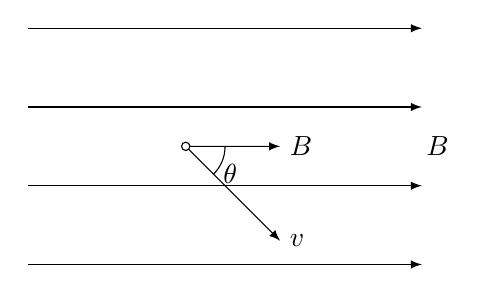
\begin{tikzpicture}[>=latex]
\foreach \x in {.5,-.5,-1.5,1.5}
{
    \draw[->](-2,\x)--(3,\x);
}
\node at (3.2,0) {$B$};
\draw[<->](1.2,-1.2)node[right]{$v$}--(0,0)--(1.2,0)node[right]{$B$};
\draw(.5,0) arc (0:-45:.5)node[right]{$\theta$};
\draw (0,0)[fill=white] circle(1.5pt);

\end{tikzpicture}
    \caption{}
    \end{minipage}
    \begin{minipage}[t]{0.48\textwidth}
    \centering
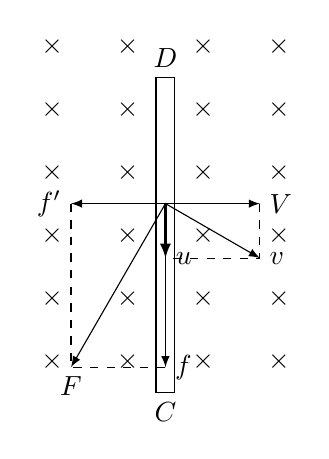
\begin{tikzpicture}[>=latex, scale=.8]
    \foreach \x in {-1.8,-.6,.6,1.8}
\foreach \y in {1,2,...,6}
{
    \node at (\x,\y){$\times$};
}
\draw (-.15,.5) rectangle (.15,5.5);
\node at (0,.5)[below]{$C$};
\node at (0,5.5)[above]{$D$};

\draw[<->](-1.5,3.5)node[left]{$f'$}--(1.5,3.5)node[right]{$V$};
\draw[<->](1.5,2.6345)node[right]{$v$}--(0,3.5)--(-1.5,0.902)node[below]{$F$};

\draw[dashed](-1.5,3.5)--(-1.5,0.902)--(0,0.902);
\draw[dashed](1.5,3.5)--(1.5,2.6345)--(0,2.6345);
\draw[->, thick](0,3.5)--(0,2.6345)node[right]{$u$};
\draw[->](0,3.5)--(0,0.902)node[right]{$f$};


\end{tikzpicture}

    \caption{}
    \end{minipage}
    \end{figure}

\subsection{产生动生电动势的能量来源}

在导体切割磁力线时,动生电动势只可能存在于运动的
这一段导体上。而不动的那一段导体上没有电动势,它只是
提供电流的通路。如果仅有一段导体在磁场中运动,而没有
回路,在这一段导线上虽然没有感生电流,但仍然可能有动生
电动势。在前一篇资料中讲过,动生电动势是由洛仑兹力引
起的。


我们知道,洛仑兹力的方向总是跟电荷的速度方向垂直
的,也就是跟电荷的运动方向垂直,所以洛仑兹力永远不对
电荷做功。而这里又说动生电动势是由洛仑兹力引起的,两者
是否矛盾?其实这并不矛盾。我们来全面考虑一下运动导体
中电子的运动。在运动导体中的电子,不但具有导体本身的
速度$V$, 而且还有相对导体的定向速度$u$, 它们的合速度为
$v$, 如图2.25所示,正是由于电子的后一种运动构成了感生
电流。电子所受的总的洛仑兹力为
\[F=evB\]
它与合速度$v$垂直,总的洛仑兹力不对电子做功。$F$的一个
分量是
\[f=eVB\]
它对电子做功,形成动生电动势;另一个分量是
\[f'=euB\]
它的方向与$V$方向相反,是阻碍导体运动的,从而做负功。可
以证明,两个分量所做的功的代数和等于零。因此,洛仑兹
力的作用并不提供能量,只是传递能量,即外力克服洛仑兹力
的一个分量$f'$所做的功通过另一个分量$f$转化为感生电流
的能量。

\subsection{公式$\mathcal{E}=B\ell v\sin\theta$ 和$\mathcal{E}=\Delta\phi/\Delta t$的关系}
课本中公式
\begin{equation}
    \mathcal{E}=B\ell v\sin\theta
\end{equation}
是作为一个特例从公式
\begin{equation}
    \mathcal{E}=\frac{\Delta\phi}{\Delta t}
\end{equation}
中推导而来的.这两个公式既有统一的一面,又
有不同的特点,因此从对比中来分析两个公式不同的方面,有
利于加深对公式的理解和正确地使用这两个公式。

从研究对象来看:公式(2.1)的研究对象是一段直导
线。$\mathcal{E}$是这段直导线在磁场中运动时产生的电动势的大小,
$\mathcal{E}$是属于这段直导线的.公式(2.2)的研究对象是一个闭合回路,
$\mathcal{E}$是通过回路的磁通量变化时在回路中产生的电动势,一般
说来$\mathcal{E}$属于整个闭合回路,如果没有附加条件,则不能求出回
路各段的电动势。

从物理内容来看,公式(2.1)是研究导线在磁场中运动
时产生的电动势,是动生电动势,它的产生是由洛仑兹力引起
的.公式(2.2)是研究通过闭合回路磁通量变化时产生的电动
势,引起磁通量变化有多种多样的原因,归纳起来不外有下述
三种类型:
\begin{enumerate}
\item 回路在$B$一定的匀强磁场中运动(包括回路的
平动,转动及回路变形,面积变化等),这样产生的是动生电动
势。
\item 回路不运动但磁场随时间变化,这样产生的电动势是
感生电动势。其本质是感应电场力充当非静电力。
\item 回路在
磁场中运动,同时磁场也随着时间变化。这时产生的电动势
是动生电动势与感生电动势之和.
\end{enumerate}


\begin{figure}[htp]
    \centering
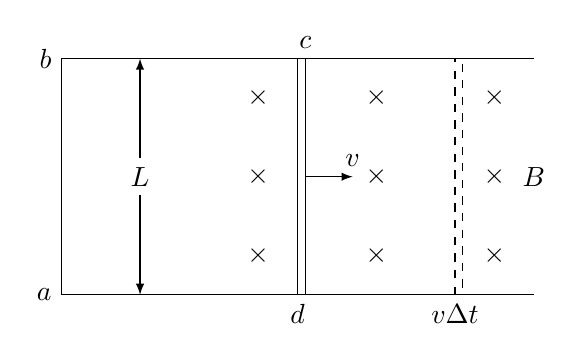
\begin{tikzpicture}[>=latex]
\draw(6,3)--(0,3)node[left]{$b$}--(0,0)node[left]{$a$}--(6,0);
\draw[<->](1,0)--node[fill=white]{$L$}(1,3);
\draw (3,0)node[below]{$d$} rectangle (3.1,3)node[above]{$c$};
\draw[->](3.1,1.5)--(3.7,1.5)node[above]{$v$};
\draw[dashed] (5,0)node[below]{$v\Delta t$}  rectangle (5.1,3);
\node at (6,1.5){$B$};
\foreach \x in {3,4.5,6}
\foreach \y in {.5,1.5,2.5}
{
    \node at (\x-.5,\y){$\times$};
}



\end{tikzpicture}
    \caption{}
\end{figure}

如图2.26所示,杆$cd$在
导轨上匀速运动,$L$、$v$均已知。磁感应强度$B$随时间均匀增
大,即$B=kt$. $t$时刻回路面积为$S$. 则在$t$到$t+\Delta t$这段时间
内磁通量的变化 
\[\Delta\phi =k(t+\Delta t)(S+Lv\Delta t)-ktS=ktLv\Delta t
+kS\Delta t+kLv(\Delta t)^2\]
则电动势为:
\[\mathcal{E}=\frac{\Delta\phi}{\Delta t}=ktLv
+kS+kLv\Delta t\]
在$\Delta t$很小时,可略去$kLv\Delta t$这一项。$ktLv$就是动生电
动势$\mathcal{E}_{\text{动}}$,$kS$就是感生电动势$\mathcal{E}_{\text{感}}$. 如果杆不动,则$\mathcal{E}_{\text{动}}=0$, 此
时$\mathcal{E}=\mathcal{E}_{\text{感}}=kS$。

从适用范围来看:公式(2.1)只适于求动生电动势,不
能求感生电动势.公式(2.2)既可求动生电动势,又可求感生电
动势,其适用范围较广.从公式(2.2)可推导公式(2.1), 反之也可
以从公式(2.1)推导公式(2.2), 这说明了两个公式的统一性.但
这种推导是有条件的,也就是必须保持磁场不随时间变化。一
般说来,公式(2.2)是由实验得到的,不能由公式(2.1)导出.课本
中强调公式(2.2)是有道理的.

\subsection{接通和断开电路的暂态电流}
为了理解课本中图2.25和图2.26的演示现象,必须
研究由自感现象引起的、不能忽略的接通和断开电路时的暂
态过程。

\begin{figure}[htp]\centering
    \begin{minipage}[t]{0.48\textwidth}
    \centering
    \includegraphics[scale=.6]{fig/2-27.png}
    \caption{}
    \end{minipage}
    \begin{minipage}[t]{0.48\textwidth}
    \centering
    \includegraphics[scale=.6]{fig/2-28.png}
    \caption{}
    \end{minipage}
    \end{figure}

设一回路如图2.27所示,回路中包含电动势为$\mathcal{E}$的电
源、电阻$R$、自感为$L$的线圈.将$K$合到1时,即将电源突然引
入$RL$电路,电路可简化为图2.28所示,在这个电路中,变
化的电流通过线图$L$时产生的自感电动势为
\[\mathcal{E}_L=-L\frac{\dd i}{\dd t}\]
因此,在任何时刻,电路中的总电动势为
\[\mathcal{E}+\mathcal{E}_L=\mathcal{E}-L\frac{\dd i}{\dd t}\]
根据欧姆定律可得
\[\mathcal{E}-L\frac{\dd i}{\dd t}=iR\]
即
\[L\frac{\dd i}{\dd t}+iR=\mathcal{E}\]
这个方程的解为
\[i= \frac{\mathcal{E}}{R}\left[1-\exp\left(-\frac{Rt}{L}\right)\right] \]

由此式可知,只有电路接通足够时间,在电路中才能建
立起稳定电流,其值为$i_0=\mathcal{E}/{R}$. 
当电路接通时,电路中的电流
$i$只能是逐渐地增加到$i_0$,而且
$L/R$的比值越大,增到$i_0$所需
时间就越长.因此课本中图2.25的实验中,所用自感线圈的
$L$越大,灯泡$A_1$的电阻$R$越小,电流增长越慢,演示效果就
越好。

如图2.27所示.当电流达到稳定值$i_0$后,如果将$K$迅
速拨到2的位置,即将电源从电路中撤除,此时电路中$\mathcal{E}=0$, 
则电流的衰减由下述方程决定
\[L\frac{\dd i}{\dd t}+iR=0\]
这个微分方程的解为
\[i=\frac{\mathcal{E}}{R}\exp\left(-\frac{Rt}{L}\right)\]
或为
\[i=i_0 \exp\left(-\frac{Rt}{L}\right)\]

上述表明,断开电源时,暂态电流是按指数规律衰减的,
虽然电源已被切断,但电路中的电流不立刻停止。

根据暂态电流的衰减规律,我们来说明课本中图2.26的
实验。设自感线圈$L$的电阻为$R_0$, 灯$A$的电阻为$R$, 因一般
$R_0\ll R$, 因此可设$R=nR_0$. 在电流稳定时,如果通过$R$的电流
为$I_1$, 通过$L$的电流为$I_2$. 因$L$与$R$并联,则$I_2R_0=I_1R$, 可得
$I_2=nI_1$. 当电源突然断开时,原来通过$R$的$I_1$立即消失.但
是,由于线圈$L$和灯泡$A$成为一个闭合电路,从而有暂态电流
$I'$存在。显然,
\[I'=I_2\cdot \exp\left(-\frac{Rt}{L}\right)\]
即
\[I'=nI_1 \exp\left(-\frac{Rt}{L}\right)\]

由此式可知,通过灯泡$A$的电流$I'$, 它的最大值$I'_{m}=nI_1$. 
因此在电路断开后的一个暂短时间内,$I'$可以超过原来通过
它的电流$I_1$, 从而灯泡亮度增加。此后,由于暂态电流随时间
迅速衰减并趋于零,灯泡才熄灭下来。如果灯泡的电阻$R$小
于线圈的电阻$R_0$, 则$I_2<I_1$, 断开后暂态电流从$I_2$开始衰减,
就不会有大于原来电流$I_1$的时候,也就不会出现灯泡更亮的
现象。可见,要做好这一演示实验,必须使灯泡电阻$R$大于线
圈电阻$R_0$, 而且
$R/R_0$
的值越大,实验效果越好。




\subsection{法拉第}

法拉第(1791—1867),英国著名物调学家和化学家。
法拉第生于伦敦一个铁匠家庭,由于家境贫苦,12岁就
当报童,后又当书店徒工,他利用业余时间学习文化知识。
1812年,法拉第听了大化学家戴维的讲演以后,产生了参加科
学工作的愿望。第二年在戴维的帮助下,进入皇家学院实验
室,作戴维的助手.1813年随戴维出访和讲学,受到了很好
的锻炼和提高.1825年任英国皇家学院实验室主任,1824年
被选为伦敦皇家学会会员,他还是法国科学院院士,1846年
他荣获伦福德奖章和皇家勋章。

法拉第在物理学方面的主要贡献是对电磁学进行了比较
系统的实验研究。他发现了电磁感应现象,总结出了电磁感
应定律,他发明了电动机和发电机,发现了电解定律,建立了
电场、磁场、力线等重要概念。

在他写成的《电学实验研究》的著作中,收集了3362个条
目,详细地记述了他做过的实验,总结出带有规律性的成果,
这是一部珍贵的科学文献。

法拉第在化学方面也做出了很大的贡献。

法拉第是靠自学成为科学家的。他在科学的征途上走了
半个多世纪,实现了自己的献身于科学的诺言。

后人为纪念法拉第,用他的名字命名电容的单位,简
称“法”。


